\chapter{Architectures}\label{Architectures}

Choosing a suitable architecture is crucial for achieving strong performance in deep learning. The choice of model defines not only the capacity for learning complex patterns, but also the inductive biases that guide generalization. In the context of \gls{ADT}, these models must operate on time-frequency representations of audio and produce accurate, frame-level onset predictions.

Each input to the model is a spectrogram of shape $(T \times D_{STFT})$, where $T$ is the sequence length (i.e., number of frames) and $D_{STFT}$ is the number of frequency bins. The corresponding output is a matrix of shape $(T \times C)$, where $C$ is the number of drum instruments being predicted.

In this thesis, I use log-magnitude spectrograms filtered with 12 logarithmically spaced, area-normalized filters per octave, spanning 20~Hz to 20,000~Hz. This results in $D_{STFT} = 84$ frequency bins. The task is to predict a common 5 class drum vocabulary, consisting of \acrfull{KD}, \acrfull{SD}, \acrfull{TT}, \acrfull{HH}, and \acrfull{CC+RC}, giving $C = 5$~\cite{zehren2024analyzingreducingsynthetictorealtransfer}.

While the input sequence length $T$ may vary, it is fixed to $T = 400$ for all experiments in this thesis, corresponding to 4 seconds of audio with 10~ms hop length. Thus, the models considered in this chapter operate with input and output shapes of $(T \times 84)$ and $(T \times 5)$, respectively.

\section{Recurrent Neural Network}

\glspl{RNN} are a foundational architecture for modeling sequential data and have demonstrated promising results on a wide range of audio-related tasks. Their core component is the \textit{recurrent unit}, which processes an input sequence one frame at a time while maintaining a hidden state that carries information from previous timesteps. This enables the model to capture temporal dependencies within the input.

To include information from both past and future frames, \glspl{RNN} can be extended to their \textit{bidirectional} variant, where one recurrent layer processes the sequence forward in time and another in reverse. This bidirectional sequential influence is illustrated in Figure~\ref{RNNInfluenceFigure}. This is particularly useful in tasks such as \gls{ADT}, where relevant auditory information may span multiple frames; for example, due to instrument timbre persisting after onset.

\begin{figure}[H]
    \centering
    \usetikzlibrary{positioning, chains, shapes.geometric, fit, shapes, arrows.meta, calc, backgrounds}

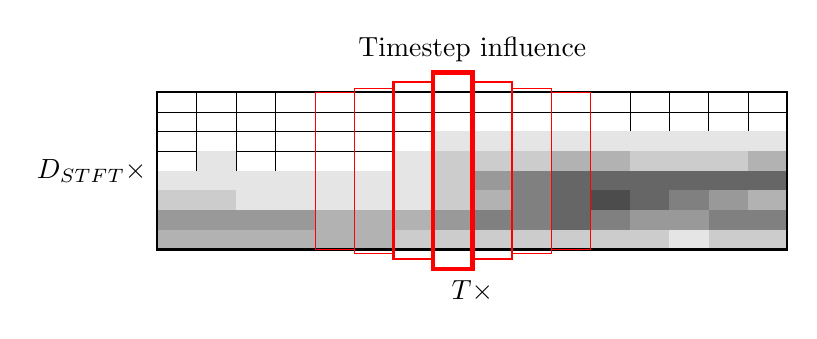
\begin{tikzpicture}[
    very thick,
    arrow/.style={
        -latex,
        very thick,
        rounded corners=0.2cm
    },
    ]

% ------ Grid ------

\draw[transform canvas={xscale=2}, step=0.25cm, ultra thin] (-2, 1) grid (2, 3);
\node[anchor=south] at (0, 3.25) {Timestep influence};
\node[anchor=east] at (-4, 2) {$D_\text{STFT}\times$};
\node[anchor=north] at (0, 0.75) {$T\times$};

% ------ Values ------

\fill[black!30] (-4.0, 1.0) rectangle (-3.5, 1.25);
\fill[black!30] (-3.5, 1.0) rectangle (-3.0, 1.25);
\fill[black!30] (-3.0, 1.0) rectangle (-2.5, 1.25);
\fill[black!30] (-2.5, 1.0) rectangle (-2.0, 1.25);
\fill[black!30] (-2.0, 1.0) rectangle (-1.5, 1.25);
\fill[black!30] (-1.5, 1.0) rectangle (-1.0, 1.25);
\fill[black!20] (-1.0, 1.0) rectangle (-0.5, 1.25);
\fill[black!20] (-0.5, 1.0) rectangle (0.0, 1.25);
\fill[black!20] (0.0, 1.0) rectangle (0.5, 1.25);
\fill[black!20] (0.5, 1.0) rectangle (1.0, 1.25);
\fill[black!20] (1.0, 1.0) rectangle (1.5, 1.25);
\fill[black!20] (1.5, 1.0) rectangle (2.0, 1.25);
\fill[black!20] (2.0, 1.0) rectangle (2.5, 1.25);
\fill[black!10] (2.5, 1.0) rectangle (3.0, 1.25);
\fill[black!20] (3.0, 1.0) rectangle (3.5, 1.25);
\fill[black!20] (3.5, 1.0) rectangle (4.0, 1.25);
\fill[black!40] (-4.0, 1.25) rectangle (-3.5, 1.5);
\fill[black!40] (-3.5, 1.25) rectangle (-3.0, 1.5);
\fill[black!40] (-3.0, 1.25) rectangle (-2.5, 1.5);
\fill[black!40] (-2.5, 1.25) rectangle (-2.0, 1.5);
\fill[black!30] (-2.0, 1.25) rectangle (-1.5, 1.5);
\fill[black!30] (-1.5, 1.25) rectangle (-1.0, 1.5);
\fill[black!30] (-1.0, 1.25) rectangle (-0.5, 1.5);
\fill[black!40] (-0.5, 1.25) rectangle (0.0, 1.5);
\fill[black!50] (0.0, 1.25) rectangle (0.5, 1.5);
\fill[black!50] (0.5, 1.25) rectangle (1.0, 1.5);
\fill[black!60] (1.0, 1.25) rectangle (1.5, 1.5);
\fill[black!50] (1.5, 1.25) rectangle (2.0, 1.5);
\fill[black!40] (2.0, 1.25) rectangle (2.5, 1.5);
\fill[black!40] (2.5, 1.25) rectangle (3.0, 1.5);
\fill[black!50] (3.0, 1.25) rectangle (3.5, 1.5);
\fill[black!50] (3.5, 1.25) rectangle (4.0, 1.5);
\fill[black!20] (-4.0, 1.5) rectangle (-3.5, 1.75);
\fill[black!20] (-3.5, 1.5) rectangle (-3.0, 1.75);
\fill[black!10] (-3.0, 1.5) rectangle (-2.5, 1.75);
\fill[black!10] (-2.5, 1.5) rectangle (-2.0, 1.75);
\fill[black!10] (-2.0, 1.5) rectangle (-1.5, 1.75);
\fill[black!10] (-1.5, 1.5) rectangle (-1.0, 1.75);
\fill[black!10] (-1.0, 1.5) rectangle (-0.5, 1.75);
\fill[black!20] (-0.5, 1.5) rectangle (0.0, 1.75);
\fill[black!30] (0.0, 1.5) rectangle (0.5, 1.75);
\fill[black!50] (0.5, 1.5) rectangle (1.0, 1.75);
\fill[black!60] (1.0, 1.5) rectangle (1.5, 1.75);
\fill[black!70] (1.5, 1.5) rectangle (2.0, 1.75);
\fill[black!60] (2.0, 1.5) rectangle (2.5, 1.75);
\fill[black!50] (2.5, 1.5) rectangle (3.0, 1.75);
\fill[black!40] (3.0, 1.5) rectangle (3.5, 1.75);
\fill[black!30] (3.5, 1.5) rectangle (4.0, 1.75);
\fill[black!10] (-4.0, 1.75) rectangle (-3.5, 2.0);
\fill[black!10] (-3.5, 1.75) rectangle (-3.0, 2.0);
\fill[black!10] (-3.0, 1.75) rectangle (-2.5, 2.0);
\fill[black!10] (-2.5, 1.75) rectangle (-2.0, 2.0);
\fill[black!10] (-2.0, 1.75) rectangle (-1.5, 2.0);
\fill[black!10] (-1.5, 1.75) rectangle (-1.0, 2.0);
\fill[black!10] (-1.0, 1.75) rectangle (-0.5, 2.0);
\fill[black!20] (-0.5, 1.75) rectangle (0.0, 2.0);
\fill[black!40] (0.0, 1.75) rectangle (0.5, 2.0);
\fill[black!50] (0.5, 1.75) rectangle (1.0, 2.0);
\fill[black!60] (1.0, 1.75) rectangle (1.5, 2.0);
\fill[black!60] (1.5, 1.75) rectangle (2.0, 2.0);
\fill[black!60] (2.0, 1.75) rectangle (2.5, 2.0);
\fill[black!60] (2.5, 1.75) rectangle (3.0, 2.0);
\fill[black!60] (3.0, 1.75) rectangle (3.5, 2.0);
\fill[black!60] (3.5, 1.75) rectangle (4.0, 2.0);
\fill[black!10] (-3.5, 2.0) rectangle (-3.0, 2.25);
\fill[black!10] (-1.0, 2.0) rectangle (-0.5, 2.25);
\fill[black!20] (-0.5, 2.0) rectangle (0.0, 2.25);
\fill[black!20] (0.0, 2.0) rectangle (0.5, 2.25);
\fill[black!20] (0.5, 2.0) rectangle (1.0, 2.25);
\fill[black!30] (1.0, 2.0) rectangle (1.5, 2.25);
\fill[black!30] (1.5, 2.0) rectangle (2.0, 2.25);
\fill[black!20] (2.0, 2.0) rectangle (2.5, 2.25);
\fill[black!20] (2.5, 2.0) rectangle (3.0, 2.25);
\fill[black!20] (3.0, 2.0) rectangle (3.5, 2.25);
\fill[black!30] (3.5, 2.0) rectangle (4.0, 2.25);
\fill[black!10] (-0.5, 2.25) rectangle (0.0, 2.5);
\fill[black!10] (0.0, 2.25) rectangle (0.5, 2.5);
\fill[black!10] (0.5, 2.25) rectangle (1.0, 2.5);
\fill[black!10] (1.0, 2.25) rectangle (1.5, 2.5);
\fill[black!10] (1.5, 2.25) rectangle (2.0, 2.5);
\fill[black!10] (2.0, 2.25) rectangle (2.5, 2.5);
\fill[black!10] (2.5, 2.25) rectangle (3.0, 2.5);
\fill[black!10] (3.0, 2.25) rectangle (3.5, 2.5);
\fill[black!10] (3.5, 2.25) rectangle (4.0, 2.5);

% ------ Outline ------
\draw[thick] (-4, 1) -- (4, 1) -- (4, 3) -- (-4, 3) -- cycle;

% ------ Influence ------

\draw[ultra thick, color=red] (-0.5, 0.75) -- (0, 0.75) -- (0, 3.25) -- (-0.5, 3.25) -- cycle;

\draw[thick, color=red] (-1, 0.875) -- (-0.5, 0.875) -- (-0.5, 3.125) -- (-1, 3.125) -- cycle;
\draw[thick, color=red] (0, 0.875) -- (0.5, 0.875) -- (0.5, 3.125) -- (0, 3.125) -- cycle;

\draw[thin, color=red] (-1.5, 0.95) -- (-1, 0.95) -- (-1, 3.05) -- (-1.5, 3.05) -- cycle;
\draw[thin, color=red] (0.5, 0.95) -- (1, 0.95) -- (1, 3.05) -- (0.5, 3.05) -- cycle;

\draw[ultra thin, color=red] (-2, 1) -- (-1.5, 1) -- (-1.5, 3) -- (-2, 3) -- cycle;
\draw[ultra thin, color=red] (1, 1) -- (1.5, 1) -- (1.5, 3) -- (1, 3) -- cycle;

\end{tikzpicture}
    \caption{Illustration of how bidirectional \glspl{RNN} include information from surrounding timesteps when predicting the current frame. The background represents a mock spectrogram of shape $(T \times D_{STFT})$, and the red boxes indicate the relative temporal influence on the middle frame. Box height reflects influence strength, gradually tapering off as distance from the center sequentially increases.}
    \label{RNNInfluenceFigure}
\end{figure}

Despite their effectiveness, traditional \glspl{RNN} suffer from the \textit{vanishing gradient problem}, which limits their ability to learn long-range dependencies. To address this, more advanced variants have been proposed, including the \gls{GRU} by Cho et al.~\cite{DBLP:conf/emnlp/ChoMGBBSB14} and the \gls{LSTM} by Hochreiter and Schmidhuber~\cite{10.1162/neco.1997.9.8.1735}.

Both \glspl{GRU} and \glspl{LSTM} have been successfully applied to \gls{ADT}-related tasks~\cite{Southall2016AutomaticDT, vogl2016recurrent, Vogl2017DrumTV, signals4040042}.

\subsection{Implementation}

I implemented the \gls{RNN} architecture using a stack of \glspl{BiRU}, followed by a frame-wise linear projection. These bidirectional recurrent layers extract and combine local temporal features at each time frame, allowing the model to consider both past and future context. The final linear layer then maps each resulting hidden state to onset probabilities for each of the five drum instruments. The full architecture is visualized in Figure~\ref{RNNFigure}.

As part of the model search, I experimented with both bidirectional \glspl{GRU} and \glspl{LSTM} as the recurrent unit, treating this choice as a tunable hyperparameter. I also varied the number of layers $L$ and the hidden size $H$. These are explicitly visualized in Table~\ref{RNNHyperparams}.

\begin{figure}[H]
    \centering
    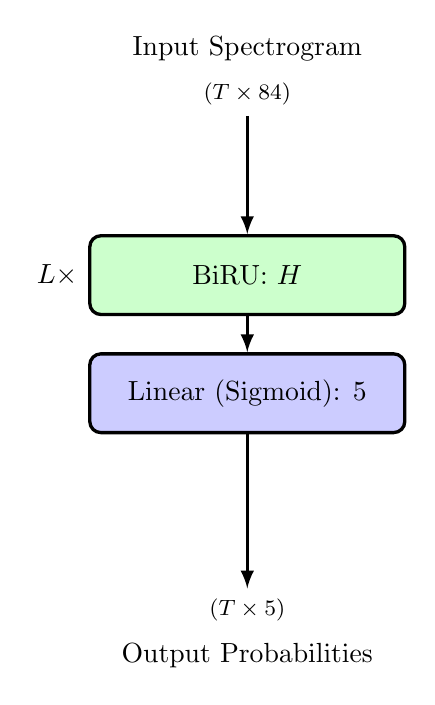
\begin{tikzpicture}[
    very thick,
    arrow/.style={
        -latex,
        very thick,
        rounded corners=0.2cm
    },
    ]

\node[anchor=south, label=above:{Input Spectrogram}] at (0, 0){\footnotesize{($T \times 84$)}};

\draw[arrow] (0, 0) -- (0, -1.5) node[rectangle, 
rounded corners, 
draw, 
anchor=north, 
label=west:$L\times$,
fill=green!20,
minimum height=1cm,
minimum width=4cm
] (a) {\acrshort{BiRU}: $H$};

\draw[arrow] (a) -- (0, -3) node[rectangle, 
rounded corners, 
draw, 
anchor=north, 
fill=blue!20,
minimum height=1cm,
minimum width=4cm
] (b) {Linear (Sigmoid): $5$};

\draw[arrow] (b) -- (0, -6);

\node[anchor=north, label=below:{Output Probabilities}] at (0, -6){\footnotesize{($T \times 5$)}};

\end{tikzpicture}
    \caption{Model architecture of the \acrlong{RNN} used in this thesis.}
    \label{RNNFigure}
\end{figure}

\begin{table}[H]
    \centering
    \begin{tabular}{lr|c}
        \multicolumn{2}{c|}{Hyperparameter} & Values       \\
        \hline
        $L$ & Number of layers      & \{2, 3, 4, 5, 6\} \\
        $H$ & Hidden size      & \{72, 144, 288, 576\} \\
        \gls{BiRU} & \acrlong{BiRU} & \{\gls{GRU}, \gls{LSTM}\}\\
    \end{tabular}
    \caption{Hyperparameters and their corresponding search spaces for training the \acrlong{RNN}.}
    \label{RNNHyperparams}
\end{table}

\section{Convolutional Neural Network}

Although spectrograms are often processed as time sequences, we've seen that they also naturally resemble images, with time and frequency forming the horizontal and vertical axes. This makes them well-suited for \glspl{CNN}, which are designed to extract local patterns in data.

A \gls{CNN} operates by applying learnable filters, called \textit{kernels}, across the input. These filters aggregate spatially local information, allowing each output unit to incorporate context from its surrounding region. When applied to spectrograms, convolutional layers enable the model to detect patterns in time-frequency space (illustrated in Figure~\ref{CNNInfluenceFigure}). This makes them a strong candidate for tasks like \gls{ADT}, where relevant features often span multiple adjacent time frames and frequency bins.

\glspl{CNN} have also been shown to perform well in \gls{ADT}, likely because this contextual information helps the model more easily learn the characteristics of instrument onsets. They are also relatively efficient to train and run, which may also help explain their reasonable performance~\cite{Vogl2017DrumTV}.

\begin{figure}[H]
    \centering
    \begin{tikzpicture}[
    very thick,
    arrow/.style={
        -latex,
        very thick,
        rounded corners=0.2cm
    },
    ]

% ------ Grid ------

\draw[transform canvas={xscale=2}, step=0.25cm, ultra thin] (-2, 1) grid (2, 3);
\node[anchor=south] at (0, 3.25) {Contextual influence};
\node[anchor=east] at (-4, 2) {$D_\text{STFT}\times$};
\node[anchor=north] at (0, 0.75) {$T\times$};

% ------ Values ------

\fill[black!30] (-4.0, 1.0) rectangle (-3.5, 1.25);
\fill[black!30] (-3.5, 1.0) rectangle (-3.0, 1.25);
\fill[black!30] (-3.0, 1.0) rectangle (-2.5, 1.25);
\fill[black!30] (-2.5, 1.0) rectangle (-2.0, 1.25);
\fill[black!30] (-2.0, 1.0) rectangle (-1.5, 1.25);
\fill[black!30] (-1.5, 1.0) rectangle (-1.0, 1.25);
\fill[black!20] (-1.0, 1.0) rectangle (-0.5, 1.25);
\fill[black!20] (-0.5, 1.0) rectangle (0.0, 1.25);
\fill[black!20] (0.0, 1.0) rectangle (0.5, 1.25);
\fill[black!20] (0.5, 1.0) rectangle (1.0, 1.25);
\fill[black!20] (1.0, 1.0) rectangle (1.5, 1.25);
\fill[black!20] (1.5, 1.0) rectangle (2.0, 1.25);
\fill[black!20] (2.0, 1.0) rectangle (2.5, 1.25);
\fill[black!10] (2.5, 1.0) rectangle (3.0, 1.25);
\fill[black!20] (3.0, 1.0) rectangle (3.5, 1.25);
\fill[black!20] (3.5, 1.0) rectangle (4.0, 1.25);
\fill[black!40] (-4.0, 1.25) rectangle (-3.5, 1.5);
\fill[black!40] (-3.5, 1.25) rectangle (-3.0, 1.5);
\fill[black!40] (-3.0, 1.25) rectangle (-2.5, 1.5);
\fill[black!40] (-2.5, 1.25) rectangle (-2.0, 1.5);
\fill[black!30] (-2.0, 1.25) rectangle (-1.5, 1.5);
\fill[black!30] (-1.5, 1.25) rectangle (-1.0, 1.5);
\fill[black!30] (-1.0, 1.25) rectangle (-0.5, 1.5);
\fill[black!40] (-0.5, 1.25) rectangle (0.0, 1.5);
\fill[black!50] (0.0, 1.25) rectangle (0.5, 1.5);
\fill[black!50] (0.5, 1.25) rectangle (1.0, 1.5);
\fill[black!60] (1.0, 1.25) rectangle (1.5, 1.5);
\fill[black!50] (1.5, 1.25) rectangle (2.0, 1.5);
\fill[black!40] (2.0, 1.25) rectangle (2.5, 1.5);
\fill[black!40] (2.5, 1.25) rectangle (3.0, 1.5);
\fill[black!50] (3.0, 1.25) rectangle (3.5, 1.5);
\fill[black!50] (3.5, 1.25) rectangle (4.0, 1.5);
\fill[black!20] (-4.0, 1.5) rectangle (-3.5, 1.75);
\fill[black!20] (-3.5, 1.5) rectangle (-3.0, 1.75);
\fill[black!10] (-3.0, 1.5) rectangle (-2.5, 1.75);
\fill[black!10] (-2.5, 1.5) rectangle (-2.0, 1.75);
\fill[black!10] (-2.0, 1.5) rectangle (-1.5, 1.75);
\fill[black!10] (-1.5, 1.5) rectangle (-1.0, 1.75);
\fill[black!10] (-1.0, 1.5) rectangle (-0.5, 1.75);
\fill[black!20] (-0.5, 1.5) rectangle (0.0, 1.75);
\fill[black!30] (0.0, 1.5) rectangle (0.5, 1.75);
\fill[black!50] (0.5, 1.5) rectangle (1.0, 1.75);
\fill[black!60] (1.0, 1.5) rectangle (1.5, 1.75);
\fill[black!70] (1.5, 1.5) rectangle (2.0, 1.75);
\fill[black!60] (2.0, 1.5) rectangle (2.5, 1.75);
\fill[black!50] (2.5, 1.5) rectangle (3.0, 1.75);
\fill[black!40] (3.0, 1.5) rectangle (3.5, 1.75);
\fill[black!30] (3.5, 1.5) rectangle (4.0, 1.75);
\fill[black!10] (-4.0, 1.75) rectangle (-3.5, 2.0);
\fill[black!10] (-3.5, 1.75) rectangle (-3.0, 2.0);
\fill[black!10] (-3.0, 1.75) rectangle (-2.5, 2.0);
\fill[black!10] (-2.5, 1.75) rectangle (-2.0, 2.0);
\fill[black!10] (-2.0, 1.75) rectangle (-1.5, 2.0);
\fill[black!10] (-1.5, 1.75) rectangle (-1.0, 2.0);
\fill[black!10] (-1.0, 1.75) rectangle (-0.5, 2.0);
\fill[black!20] (-0.5, 1.75) rectangle (0.0, 2.0);
\fill[black!40] (0.0, 1.75) rectangle (0.5, 2.0);
\fill[black!50] (0.5, 1.75) rectangle (1.0, 2.0);
\fill[black!60] (1.0, 1.75) rectangle (1.5, 2.0);
\fill[black!60] (1.5, 1.75) rectangle (2.0, 2.0);
\fill[black!60] (2.0, 1.75) rectangle (2.5, 2.0);
\fill[black!60] (2.5, 1.75) rectangle (3.0, 2.0);
\fill[black!60] (3.0, 1.75) rectangle (3.5, 2.0);
\fill[black!60] (3.5, 1.75) rectangle (4.0, 2.0);
\fill[black!10] (-3.5, 2.0) rectangle (-3.0, 2.25);
\fill[black!10] (-1.0, 2.0) rectangle (-0.5, 2.25);
\fill[black!20] (-0.5, 2.0) rectangle (0.0, 2.25);
\fill[black!20] (0.0, 2.0) rectangle (0.5, 2.25);
\fill[black!20] (0.5, 2.0) rectangle (1.0, 2.25);
\fill[black!30] (1.0, 2.0) rectangle (1.5, 2.25);
\fill[black!30] (1.5, 2.0) rectangle (2.0, 2.25);
\fill[black!20] (2.0, 2.0) rectangle (2.5, 2.25);
\fill[black!20] (2.5, 2.0) rectangle (3.0, 2.25);
\fill[black!20] (3.0, 2.0) rectangle (3.5, 2.25);
\fill[black!30] (3.5, 2.0) rectangle (4.0, 2.25);
\fill[black!10] (-0.5, 2.25) rectangle (0.0, 2.5);
\fill[black!10] (0.0, 2.25) rectangle (0.5, 2.5);
\fill[black!10] (0.5, 2.25) rectangle (1.0, 2.5);
\fill[black!10] (1.0, 2.25) rectangle (1.5, 2.5);
\fill[black!10] (1.5, 2.25) rectangle (2.0, 2.5);
\fill[black!10] (2.0, 2.25) rectangle (2.5, 2.5);
\fill[black!10] (2.5, 2.25) rectangle (3.0, 2.5);
\fill[black!10] (3.0, 2.25) rectangle (3.5, 2.5);
\fill[black!10] (3.5, 2.25) rectangle (4.0, 2.5);

% ------ Outline ------
\draw[thick] (-4, 1) -- (4, 1) -- (4, 3) -- (-4, 3) -- cycle;

% ------ Influence ------

\draw[ultra thick, color=red, pattern=north east lines, pattern color=red] (-0.5, 1) -- (0, 1) -- (0, 3) -- (-0.5, 3) -- cycle;

\draw[thick, color=red] (-1, 1) -- (0.5, 1) -- (0.5, 3.) -- (-1, 3) -- cycle;


\end{tikzpicture}
    \caption{Illustration of how \glspl{CNN} use a fixed-size receptive field to incorporate local context from surrounding time frames. The background represents a mock spectrogram. The red shaded region marks the center time frame being predicted, and the red boxes indicate the receptive field, the neighboring frames that influence the prediction.}
    \label{CNNInfluenceFigure}
\end{figure}

\subsection{Implementation}

My \gls{CNN} architecture begins with $I$ initial convolutional blocks, each designed to preserve the temporal resolution of the input, ensuring that the output retains the same sequence length $T$. Within these blocks, the number of kernels $K_i$ increases with block depth $i$, using $K = \{32, 64, 96\}$ to enable deeper layers to capture more complex time–frequency patterns. This kernel progression is fixed (i.e., not treated as a hyperparameter), and follows a common design convention of increasing the filter count with depth~\cite{simonyan2014very}.

These convolutional blocks iteratively combine local features from the spectrogram, forming a richer internal representation of the input. This representation is then passed through $L$ fully connected layers, which project the features into an $H$-dimensional latent space for final interpretation. 

Each convolutional and fully connected layer is followed by a \gls{ReLU} activation function. Finally, an output layer computes onset probabilities for each of the five drum instruments. The architecture is visualized in Figure~\ref{CNNFigure}, with tunable hyperparameters stated in Table~\ref{CNNHyperparams}.

\begin{figure}[H]
    \centering
    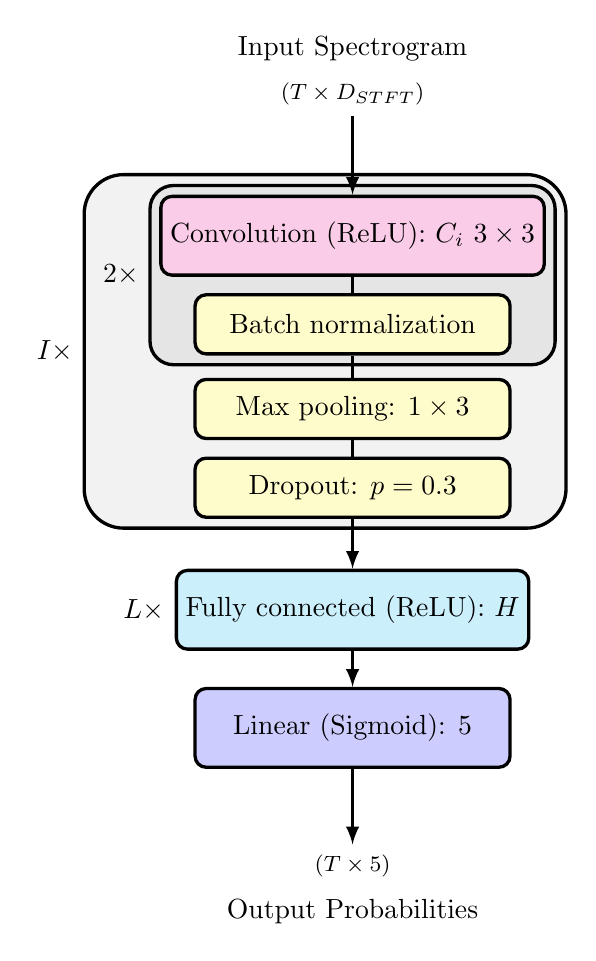
\begin{tikzpicture}[
    very thick,
    arrow/.style={
        -latex,
        very thick,
        rounded corners=0.2cm
    },
    ]

\node[anchor=south, label=above:{Input Spectrogram}] at (0, -0.5){\footnotesize{($T \times D_\text{STFT}$)}};

\draw[arrow] (0, -0.5) -- (0, -1.5) node [rectangle,
rounded corners,
draw,
anchor=north,
fill=magenta!20,
minimum height=1cm,
minimum width=4cm
] (a) {Convolution (ReLU): $C_i$  $3 \times 3$};

\draw (a) -- (0, -2.75) node[rectangle,
rounded corners,
draw,
anchor=north,
fill=yellow!20,
minimum height=0.75cm,
minimum width=4cm
] (b) {Batch normalization};

\draw (b) -- (0, -3.825) node[rectangle,
rounded corners,
draw,
anchor=north,
fill=yellow!20,
minimum height=0.75cm,
minimum width=4cm
] (c) {Max pooling: $1 \times 3$};

\draw (c) -- (0, -4.825) node[rectangle,
rounded corners,
draw,
anchor=north,
fill=yellow!20,
minimum height=0.75cm,
minimum width=4cm
] (d) {Dropout: $p = 0.3$};

\begin{scope}[on background layer]
    \node[rectangle,
    fill=gray!20,
    rounded corners=3mm,
    label={[name=ablabel]west:$2\times$},
    draw,
    very thick,
    fit=(a) (b)] (ab) {};
    \node[rectangle,
    fill=gray!10,
    rounded corners=5mm,
    label=west:$I\times$,
    draw,
    very thick,
    fit= (ab) (ablabel) (d)] {};
    \node[rectangle,
    fill=gray!20,
    rounded corners=3mm,
    label={[name=ablabel]west:$2\times$},
    draw,
    very thick,
    fit=(a) (b)] (ab) {};
\end{scope}


\draw[arrow] (d) -- (0, -6.25) node[rectangle, 
rounded corners, 
draw, 
anchor=north, 
label=west:$L\times$,
fill=cyan!20,
minimum height=1cm,
minimum width=4cm
] (g) {Fully connected (ReLU): $H$};

\draw[arrow] (g) -- (0, -7.75) node[rectangle, 
rounded corners, 
draw, 
anchor=north, 
fill=blue!20,
minimum height=1cm,
minimum width=4cm
] (h) {Linear (Sigmoid): $5$};

\draw[arrow] (h) -- (0, -9.75);

\node[anchor=north, label=below:{Output Probabilities}] at (0, -9.75){\footnotesize{($T \times 5$)}};

\end{tikzpicture}
    \caption{Model architecture of the \acrlong{CNN} used in this thesis.}
    \label{CNNFigure}
\end{figure}

\begin{table}[H]
    \centering
    \begin{tabular}{lr|c}
        \multicolumn{2}{c|}{Hyperparameter} & Values       \\
        \hline
        $I$ & Number of convolutions & \{1, 2, 3\}\\
        $L$ & Number of layers      & \{2, 3, 4\} \\
        $H$ & Hidden size      & \{72, 144, 288, 576\} \\
    \end{tabular}
    \caption{Hyperparameters and their corresponding search spaces for training the \acrlong{CNN}.}
    \label{CNNHyperparams}
\end{table}

\section[Convolutional RNN]{Convolutional Recurrent Neural Network}

The strengths of the recurrent layers and convolutions are not mutually exclusive. Theoretically, they can harmonize when combined into a unified architecture, the \gls{CRNN}, where each component complements the other.

Intuitively, the ability of \glspl{CNN} to extract local time–frequency patterns from spectrograms, together with the ability of \glspl{RNN} to model temporal dependencies, makes this combination particularly well-suited for \gls{ADT}. This merging of contextual representation and cross-timestep memory has shown promising results in prior work~\cite{Vogl2017DrumTV, vogl2018multiinstrumentdrumtranscription, signals4040042}.

\subsection{Implementation}

I implemented the \gls{CRNN} using a fixed stack of $I = 2$ initial convolutional blocks, a setup inspired by prior work in \gls{ADT}~\cite{Vogl2017DrumTV, signals4040042}. These convolutional blocks use an increasing number of kernels $K = \{32, 64\}$, allowing deeper layers to extract more complex time–frequency patterns. As with the pure \gls{CNN}, the convolutions preserve the input's temporal resolution.

The resulting convolutional output is passed to a \gls{BiRU}, which models temporal dependencies across frames. As in the \gls{RNN} architecture, I experimented with both \glspl{GRU} and \glspl{LSTM}. Each timestep's hidden state is then passed into the final linear layer, which computes and outputs onset probabilities for each of the five drum instruments. The full architecture can be seen in Figure~\ref{CRNNFigure}, with its corresponding tunable hyperparameters in Table~\ref{CRNNHyperparams}.

\begin{figure}[H]
    \centering
    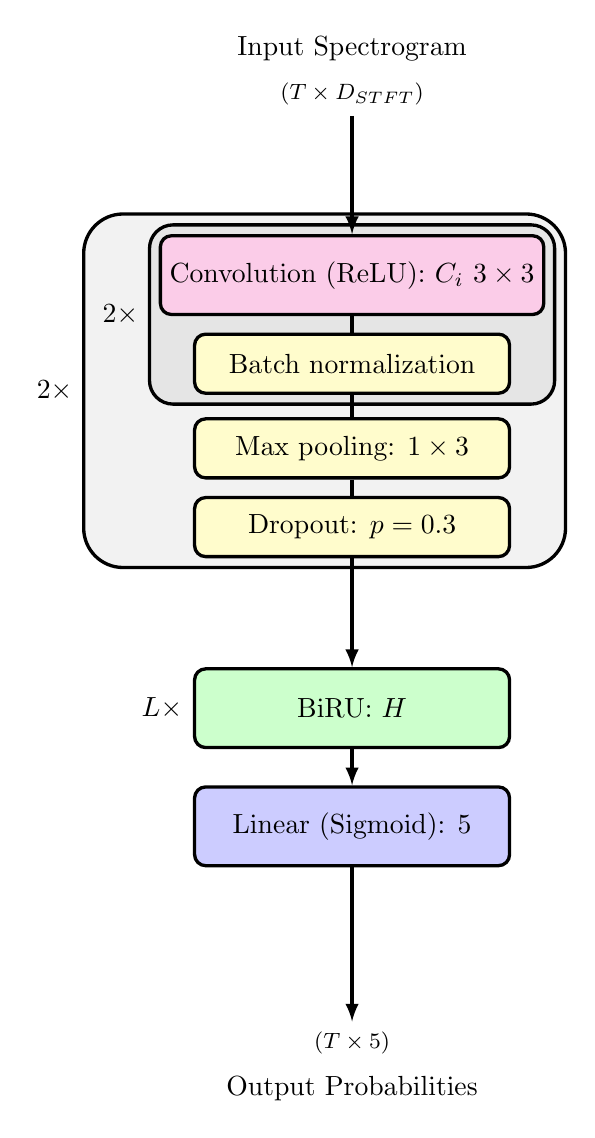
\begin{tikzpicture}[
    very thick,
    arrow/.style={
        -latex,
        very thick,
        rounded corners=0.2cm
    },
    ]

\node[anchor=south, label=above:{Input Spectrogram}] at (0, 0){\footnotesize{($T \times D_\text{STFT}$)}};

\draw[arrow] (0, 0) -- (0, -1.5) node [rectangle,
rounded corners,
draw,
anchor=north,
fill=magenta!20,
minimum height=1cm,
minimum width=4cm
] (a) {Convolution (ReLU): $C_i$  $3 \times 3$};

\draw (a) -- (0, -2.75) node[rectangle,
rounded corners,
draw,
anchor=north,
fill=yellow!20,
minimum height=0.75cm,
minimum width=4cm
] (b) {Batch normalization};

\draw (b) -- (0, -3.825) node[rectangle,
rounded corners,
draw,
anchor=north,
fill=yellow!20,
minimum height=0.75cm,
minimum width=4cm
] (c) {Max pooling: $1 \times 3$};

\draw (c) -- (0, -4.825) node[rectangle,
rounded corners,
draw,
anchor=north,
fill=yellow!20,
minimum height=0.75cm,
minimum width=4cm
] (d) {Dropout: $p = 0.3$};

\begin{scope}[on background layer]
    \node[rectangle,
    fill=gray!20,
    rounded corners=3mm,
    label={[name=ablabel]west:$2\times$},
    draw,
    very thick,
    fit=(a) (b)] (ab) {};
    \node[rectangle,
    fill=gray!10,
    rounded corners=5mm,
    label=west:$2\times$,
    draw,
    very thick,
    fit= (ab) (ablabel) (d)] {};
    \node[rectangle,
    fill=gray!20,
    rounded corners=3mm,
    label={[name=ablabel]west:$2\times$},
    draw,
    very thick,
    fit=(a) (b)] (ab) {};
\end{scope}

\draw[arrow] (d) -- (0, -7) node[rectangle, 
rounded corners, 
draw, 
anchor=north, 
label=west:$L\times$,
fill=green!20,
minimum height=1cm,
minimum width=4cm
] (g) {BiRU: $H$};

\draw[arrow] (g) -- (0, -8.5) node[rectangle, 
rounded corners, 
draw, 
anchor=north, 
fill=blue!20,
minimum height=1cm,
minimum width=4cm
] (h) {Linear (Sigmoid): $5$};

\draw[arrow] (h) -- (0, -11.5);

\node[anchor=north, label=below:{Output Probabilities}] at (0, -11.5){\footnotesize{($T \times 5$)}};

\end{tikzpicture}
    \caption{Model architecture of the \acrlong{CRNN} used in this thesis.}
    \label{CRNNFigure}
\end{figure}

\begin{table}[H]
    \centering
    \begin{tabular}{lr|c}
        \multicolumn{2}{c|}{Hyperparameter} & Values       \\
        \hline
        $L$ & Number of layers      & \{2, 3, 4, 5\} \\
        $H$ & Hidden size      & \{72, 144, 288, 576\} \\
        \gls{BiRU} & \acrlong{BiRU} & \{\gls{GRU}, \gls{LSTM}\}\\
    \end{tabular}
    \caption{Hyperparameters and their corresponding search spaces for training the \acrlong{CRNN}.}
    \label{CRNNHyperparams}
\end{table}

\section{Convolutional Transformer}

While \glspl{CRNN} have proven effective at combining local time–frequency pattern extraction with temporal modeling, their ability to capture long-range dependencies still remains limited. Recurrent layers often struggle to maintain distant information through their hidden states, and convolutional layers are constrained by the size of their fixed receptive field.

To address these limitations, a major architectural shift was instigated, most notably with the introduction of the \textit{attention} mechanism in Google's "Attention Is All You Need"~\cite{NIPS2017_3f5ee243}. This mechanism allows models to dynamically focus, or \textit{attend}, to different parts of an input sequence by learning relationships between its elements. Replacing recurrent layers with stacks of attention-based blocks gave rise to a new class of models: the \textit{transformers}.

Unlike recurrent units, which propagate information sequentially through hidden states, attention layers allow each timestep to directly access information from every other timestep in the sequence. This gives the model a more flexible way to capture a global context. Intuitively, it enables each element to \textit{"intelligently"} decide which other parts of the sequence it wants to focus on, rather than depending on neighbouring timesteps to pass information forward (visualized in Figure~\ref{CTInfluenceFigure}).

\begin{figure}[H]
    \centering
    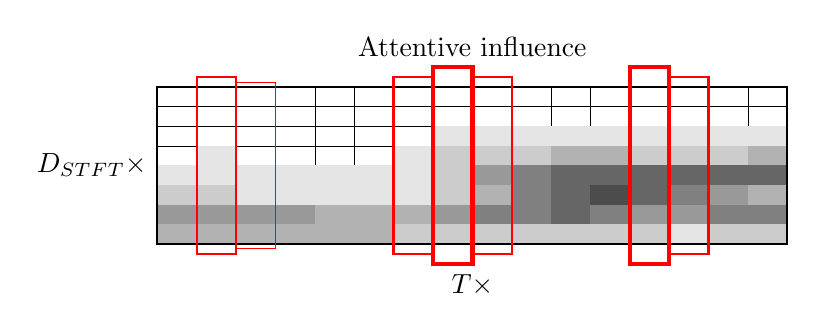
\begin{tikzpicture}[
    very thick,
    arrow/.style={
        -latex,
        very thick,
        rounded corners=0.2cm
    },
    ]

% ------ Grid ------

\draw[transform canvas={xscale=2}, step=0.25cm, ultra thin] (-2, 1) grid (2, 3);
\node[anchor=south] at (0, 3.25) {Attentive influence};
\node[anchor=east] at (-4, 2) {$D_\text{STFT}\times$};
\node[anchor=north] at (0, 0.75) {$T\times$};

% ------ Values ------

\fill[black!30] (-4.0, 1.0) rectangle (-3.5, 1.25);
\fill[black!30] (-3.5, 1.0) rectangle (-3.0, 1.25);
\fill[black!30] (-3.0, 1.0) rectangle (-2.5, 1.25);
\fill[black!30] (-2.5, 1.0) rectangle (-2.0, 1.25);
\fill[black!30] (-2.0, 1.0) rectangle (-1.5, 1.25);
\fill[black!30] (-1.5, 1.0) rectangle (-1.0, 1.25);
\fill[black!20] (-1.0, 1.0) rectangle (-0.5, 1.25);
\fill[black!20] (-0.5, 1.0) rectangle (0.0, 1.25);
\fill[black!20] (0.0, 1.0) rectangle (0.5, 1.25);
\fill[black!20] (0.5, 1.0) rectangle (1.0, 1.25);
\fill[black!20] (1.0, 1.0) rectangle (1.5, 1.25);
\fill[black!20] (1.5, 1.0) rectangle (2.0, 1.25);
\fill[black!20] (2.0, 1.0) rectangle (2.5, 1.25);
\fill[black!10] (2.5, 1.0) rectangle (3.0, 1.25);
\fill[black!20] (3.0, 1.0) rectangle (3.5, 1.25);
\fill[black!20] (3.5, 1.0) rectangle (4.0, 1.25);
\fill[black!40] (-4.0, 1.25) rectangle (-3.5, 1.5);
\fill[black!40] (-3.5, 1.25) rectangle (-3.0, 1.5);
\fill[black!40] (-3.0, 1.25) rectangle (-2.5, 1.5);
\fill[black!40] (-2.5, 1.25) rectangle (-2.0, 1.5);
\fill[black!30] (-2.0, 1.25) rectangle (-1.5, 1.5);
\fill[black!30] (-1.5, 1.25) rectangle (-1.0, 1.5);
\fill[black!30] (-1.0, 1.25) rectangle (-0.5, 1.5);
\fill[black!40] (-0.5, 1.25) rectangle (0.0, 1.5);
\fill[black!50] (0.0, 1.25) rectangle (0.5, 1.5);
\fill[black!50] (0.5, 1.25) rectangle (1.0, 1.5);
\fill[black!60] (1.0, 1.25) rectangle (1.5, 1.5);
\fill[black!50] (1.5, 1.25) rectangle (2.0, 1.5);
\fill[black!40] (2.0, 1.25) rectangle (2.5, 1.5);
\fill[black!40] (2.5, 1.25) rectangle (3.0, 1.5);
\fill[black!50] (3.0, 1.25) rectangle (3.5, 1.5);
\fill[black!50] (3.5, 1.25) rectangle (4.0, 1.5);
\fill[black!20] (-4.0, 1.5) rectangle (-3.5, 1.75);
\fill[black!20] (-3.5, 1.5) rectangle (-3.0, 1.75);
\fill[black!10] (-3.0, 1.5) rectangle (-2.5, 1.75);
\fill[black!10] (-2.5, 1.5) rectangle (-2.0, 1.75);
\fill[black!10] (-2.0, 1.5) rectangle (-1.5, 1.75);
\fill[black!10] (-1.5, 1.5) rectangle (-1.0, 1.75);
\fill[black!10] (-1.0, 1.5) rectangle (-0.5, 1.75);
\fill[black!20] (-0.5, 1.5) rectangle (0.0, 1.75);
\fill[black!30] (0.0, 1.5) rectangle (0.5, 1.75);
\fill[black!50] (0.5, 1.5) rectangle (1.0, 1.75);
\fill[black!60] (1.0, 1.5) rectangle (1.5, 1.75);
\fill[black!70] (1.5, 1.5) rectangle (2.0, 1.75);
\fill[black!60] (2.0, 1.5) rectangle (2.5, 1.75);
\fill[black!50] (2.5, 1.5) rectangle (3.0, 1.75);
\fill[black!40] (3.0, 1.5) rectangle (3.5, 1.75);
\fill[black!30] (3.5, 1.5) rectangle (4.0, 1.75);
\fill[black!10] (-4.0, 1.75) rectangle (-3.5, 2.0);
\fill[black!10] (-3.5, 1.75) rectangle (-3.0, 2.0);
\fill[black!10] (-3.0, 1.75) rectangle (-2.5, 2.0);
\fill[black!10] (-2.5, 1.75) rectangle (-2.0, 2.0);
\fill[black!10] (-2.0, 1.75) rectangle (-1.5, 2.0);
\fill[black!10] (-1.5, 1.75) rectangle (-1.0, 2.0);
\fill[black!10] (-1.0, 1.75) rectangle (-0.5, 2.0);
\fill[black!20] (-0.5, 1.75) rectangle (0.0, 2.0);
\fill[black!40] (0.0, 1.75) rectangle (0.5, 2.0);
\fill[black!50] (0.5, 1.75) rectangle (1.0, 2.0);
\fill[black!60] (1.0, 1.75) rectangle (1.5, 2.0);
\fill[black!60] (1.5, 1.75) rectangle (2.0, 2.0);
\fill[black!60] (2.0, 1.75) rectangle (2.5, 2.0);
\fill[black!60] (2.5, 1.75) rectangle (3.0, 2.0);
\fill[black!60] (3.0, 1.75) rectangle (3.5, 2.0);
\fill[black!60] (3.5, 1.75) rectangle (4.0, 2.0);
\fill[black!10] (-3.5, 2.0) rectangle (-3.0, 2.25);
\fill[black!10] (-1.0, 2.0) rectangle (-0.5, 2.25);
\fill[black!20] (-0.5, 2.0) rectangle (0.0, 2.25);
\fill[black!20] (0.0, 2.0) rectangle (0.5, 2.25);
\fill[black!20] (0.5, 2.0) rectangle (1.0, 2.25);
\fill[black!30] (1.0, 2.0) rectangle (1.5, 2.25);
\fill[black!30] (1.5, 2.0) rectangle (2.0, 2.25);
\fill[black!20] (2.0, 2.0) rectangle (2.5, 2.25);
\fill[black!20] (2.5, 2.0) rectangle (3.0, 2.25);
\fill[black!20] (3.0, 2.0) rectangle (3.5, 2.25);
\fill[black!30] (3.5, 2.0) rectangle (4.0, 2.25);
\fill[black!10] (-0.5, 2.25) rectangle (0.0, 2.5);
\fill[black!10] (0.0, 2.25) rectangle (0.5, 2.5);
\fill[black!10] (0.5, 2.25) rectangle (1.0, 2.5);
\fill[black!10] (1.0, 2.25) rectangle (1.5, 2.5);
\fill[black!10] (1.5, 2.25) rectangle (2.0, 2.5);
\fill[black!10] (2.0, 2.25) rectangle (2.5, 2.5);
\fill[black!10] (2.5, 2.25) rectangle (3.0, 2.5);
\fill[black!10] (3.0, 2.25) rectangle (3.5, 2.5);
\fill[black!10] (3.5, 2.25) rectangle (4.0, 2.5);

% ------ Outline ------
\draw[thick] (-4, 1) -- (4, 1) -- (4, 3) -- (-4, 3) -- cycle;

% ------ Influence ------

\draw[ultra thick, color=red] (-0.5, 0.75) -- (0, 0.75) -- (0, 3.25) -- (-0.5, 3.25) -- cycle;
\draw[ultra thick, color=red] (2, 0.75) -- (2.5, 0.75) -- (2.5, 3.25) -- (2, 3.25) -- cycle;


\draw[thick, color=red] (2.5, 0.875) -- (3, 0.875) -- (3, 3.125) -- (2.5, 3.125) -- cycle;
%\draw[thick, color=red] (1.5, 0.875) -- (2, 0.875) -- (2, 3.125) -- (1.5, 3.125) -- cycle;
\draw[thick, color=red] (0, 0.875) -- (0.5, 0.875) -- (0.5, 3.125) -- (0, 3.125) -- cycle;
\draw[thick, color=red] (-1, 0.875) -- (-0.5, 0.875) -- (-0.5, 3.125) -- (-1, 3.125) -- cycle;
\draw[thick, color=red] (-3.5, 0.875) -- (-3, 0.875) -- (-3, 3.125) -- (-3.5, 3.125) -- cycle;
%\draw[thick, color=red] (-3, 0.875) -- (-2.5, 0.875) -- (-2.5, 3.125) -- (-3, 3.125) -- cycle;

\draw[thin, color=red] (-3, 0.95) -- (-2.5, 0.95) -- (-2.5, 3.05) -- (-3, 3.05) -- cycle;
%\draw[thin, color=red] (3, 0.95) -- (3.5, 0.95) -- (3.5, 3.05) -- (3, 3.05) -- cycle;
%\draw[thin, color=red] (1, 0.95) -- (1.5, 0.95) -- (1.5, 3.05) -- (1, 3.05) -- cycle;
%\draw[thin, color=red] (-1.5, 0.95) -- (-1, 0.95) -- (-1, 3.05) -- (-1.5, 3.05) -- cycle;


\end{tikzpicture}
    \caption{Illustration of how attention layers enable influence from time frames across the entire sequence, regardless of their relative position. The background represents a mock spectrogram, and the red boxes indicate the time frames influencing the prediction on the middle frame. Box height reflects the relative influence strength, as determined by attention weights.}
    \label{CTInfluenceFigure}
\end{figure}

Attention mechanisms have recently shown strong performance in both \gls{AMT} and \gls{ADT}, in some cases outperforming \glspl{RNN}. Replacing recurrent layers with transformer blocks may therefore improve the model's ability to capture long-range dependencies, particularly when combined with convolutional layers that extract local time–frequency patterns~\cite{9747048, gardner2022mt3multitaskmultitrackmusic, signals4040042, chang2024yourmt3+, zehren2024analyzingreducingsynthetictorealtransfer}.

\subsection{Implementation}

I implemented the convolutional transformer architecture using an initial fixed stack of $I = 2$ convolutional blocks, following the same configuration as in the \gls{CRNN}. These blocks use an increasing number of kernels $K = \{32, 64\}$, as in the \gls{CRNN} setup. 

The convolutional output is then projected into a lower-dimensional embedding space of size $D_e$, which reduces computational load and acts as input to the transformer blocks. A sinusoidal positional encoding is added to this embedding to provide the model with temporal ordering information, compensating for the transformer's lack of inherent sequence structure. 

The core of the model consists of $L$ transformer blocks with pre-layer normalization, a design shown to improve training stability compared to post-layer normalization~\cite{pmlr-v119-xiong20b}. Each block contains multi-head self-attention with $H$ heads, enabling the model to capture global dependencies across the input sequence. The first layer of each block's feedforward component uses the \gls{GELU} activation function, which is standard in transformer-based models and has shown improved performance over \gls{ReLU}~\cite{devlin-etal-2019-bert, hendrycks2023gaussianerrorlinearunits}. 

Finally, a linear output layer computes onset probabilities for each of the five drum instruments. Figure~\ref{CTFigure} illustrates the whole convolutional transformer architecture, with its tunable hyperparameters shown in Table~\ref{CTHyperparams}.

\begin{figure}[H]
    \centering
    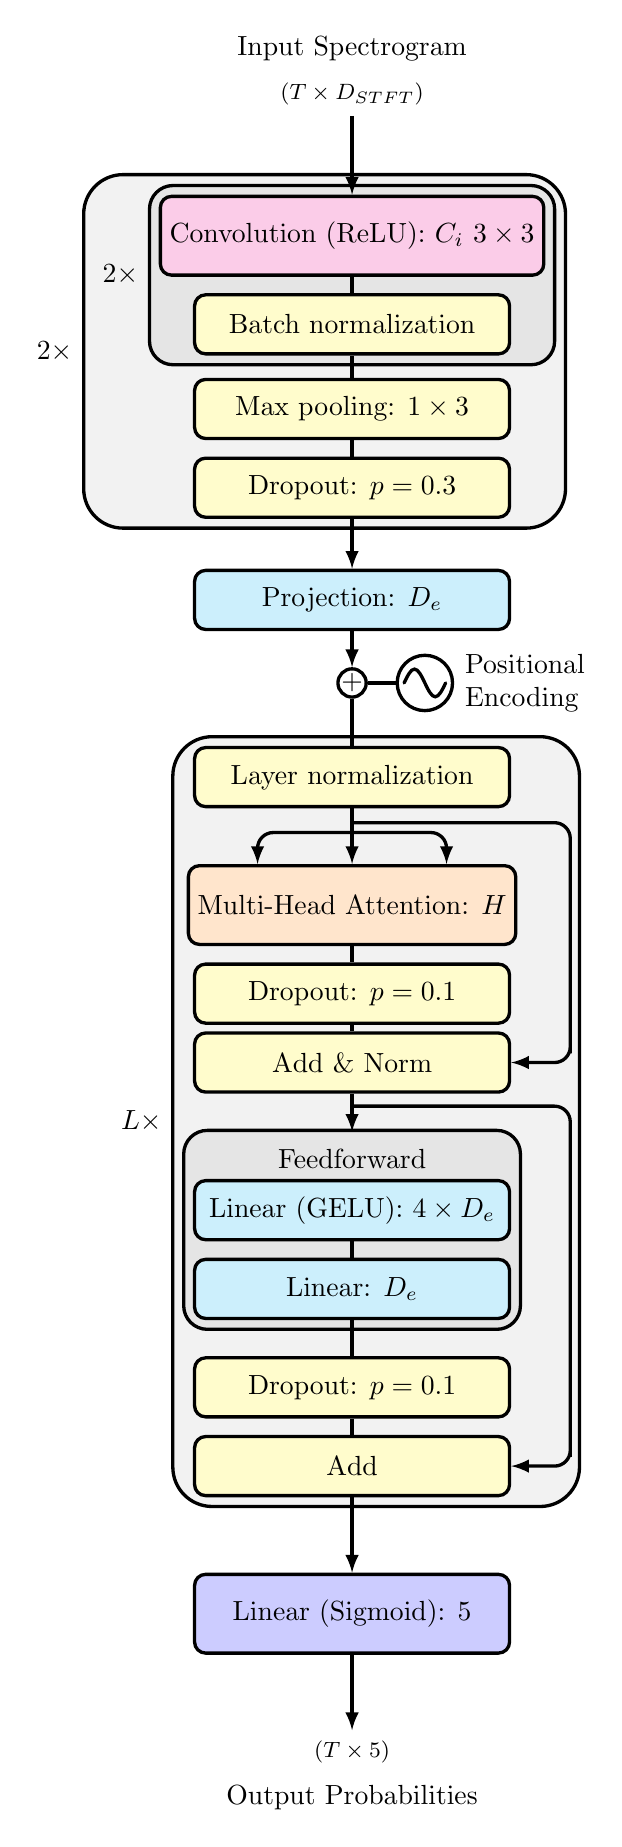
\begin{tikzpicture}[
    very thick,
    arrow/.style={
        -latex,
        very thick,
        rounded corners=0.2cm
    },
    do path picture/.style={%
        path picture={%
          \pgfpointdiff{\pgfpointanchor{path picture bounding box}{south west}}%
            {\pgfpointanchor{path picture bounding box}{north east}}%
          \pgfgetlastxy\x\y%
          \tikzset{x=\x/2,y=\y/2}%
          #1
        }
    },
    sin wave/.style={do path picture={    
        \draw [line cap=round] (-3/4,0)
        sin (-3/8,1/2) cos (0,0) sin (3/8,-1/2) cos (3/4,0);
        }
    }
    ]

\node[anchor=south, label=above:{Input Spectrogram}] at (0, -0.5){\footnotesize{($T \times D_\text{STFT}$)}};

\draw[arrow] (0, -0.5) -- (0, -1.5) node [rectangle,
rounded corners,
draw,
anchor=north,
fill=magenta!20,
minimum height=1cm,
minimum width=4cm
] (a) {Convolution (ReLU): $C_i$  $3 \times 3$};

\draw (a) -- (0, -2.75) node[rectangle,
rounded corners,
draw,
anchor=north,
fill=yellow!20,
minimum height=0.75cm,
minimum width=4cm
] (b) {Batch normalization};

\draw (b) -- (0, -3.825) node[rectangle,
rounded corners,
draw,
anchor=north,
fill=yellow!20,
minimum height=0.75cm,
minimum width=4cm
] (c) {Max pooling: $1 \times 3$};

\draw (c) -- (0, -4.825) node[rectangle,
rounded corners,
draw,
anchor=north,
fill=yellow!20,
minimum height=0.75cm,
minimum width=4cm
] (d) {Dropout: $p = 0.3$};

\begin{scope}[on background layer]
    \node[rectangle,
    fill=gray!20,
    rounded corners=3mm,
    label={[name=ablabel]west:$2\times$},
    draw,
    very thick,
    fit=(a) (b)] (ab) {};
    \node[rectangle,
    fill=gray!10,
    rounded corners=5mm,
    label=west:$2\times$,
    draw,
    very thick,
    fit= (ab) (ablabel) (d)] {};
    \node[rectangle,
    fill=gray!20,
    rounded corners=3mm,
    label={[name=ablabel]west:$2\times$},
    draw,
    very thick,
    fit=(a) (b)] (ab) {};
\end{scope};

\draw[arrow] (d) -- (0, -6.25) node[rectangle,
rounded corners,
draw,
anchor=north,
fill=cyan!20,
minimum height=0.75cm,
minimum width=4cm
] (g) {Projection: $D_e$};

\draw[arrow] (g) -- (0, -7.5) node[circle, 
draw, 
anchor=north,
minimum size=1em, 
inner sep=0pt
] (h) {$\mathbf{+}$};

\node [circle, 
draw, 
sin wave, 
minimum size=2em, 
right=1em of h,
label={[align=left]east:Positional\\Encoding},
] (pe) {};

\draw (pe) -- (h);

\draw (h) -- (0, -8.5) node[rectangle,
rounded corners,
draw,
anchor=north,
fill=yellow!20,
minimum height=0.75cm,
minimum width=4cm
] (i) {Layer normalization};

\draw[arrow] (i) -- (0, -10) node [rectangle,
rounded corners,
draw,
anchor=north,
fill=orange!20,
minimum height=1cm,
minimum width=4cm
] (j) {Multi-Head Attention: $H$};

\draw[arrow] (j.north)++(0, 0.4) -| ($(j.north) + (1.2,0)$);
\draw[arrow] (j.north)++(0, 0.4) -| ($(j.north) + (-1.2,0)$);

\draw (j) -- (0, -11.25) node[rectangle,
rounded corners,
draw,
anchor=north,
fill=yellow!20,
minimum height=0.75cm,
minimum width=4cm
] (k) {Dropout: $p = 0.1$};

\draw (k) -- (0, -12.125) node[rectangle,
rounded corners,
draw,
anchor=north,
fill=yellow!20,
minimum height=0.75cm,
minimum width=4cm
] (l) {Add \& Norm};

\coordinate (larrow) at ($(l.east) + (0.75, 0)$);
\draw[arrow] (j.north)++(0, 0.525) -| (larrow) |- (l.east);

\node[rectangle,
rounded corners,
draw,
anchor=north,
fill=cyan!20,
minimum height=0.75cm,
minimum width=4cm
] at (0, -14) (m) {Linear (GELU): $4 \times D_e$};

\coordinate (m1) at ($(m.north) + (0, 0.5)$);
\draw[arrow] (l) -- ($(m1.north) + (0, 0.1)$);

\draw (m) -- (0, -15) node[rectangle,
rounded corners,
draw,
anchor=north,
fill=cyan!20,
minimum height=0.75cm,
minimum width=4cm
] (n) {Linear: $D_e$};

\draw (n) -- (0, -16.25) node[rectangle,
rounded corners,
draw,
anchor=north,
fill=yellow!20,
minimum height=0.75cm,
minimum width=4cm
] (o) {Dropout: $p = 0.1$};

\draw (o) -- (0, -17.25) node[rectangle,
rounded corners,
draw,
anchor=north,
fill=yellow!20,
minimum height=0.75cm,
minimum width=4cm
] (p) {Add};

\draw[arrow] (m.north)++(0, 0.925) -| ($(p.east) + (0.75, 0)$) |- (p.east);

\begin{scope}[on background layer]

    \node[rectangle,
    fill=gray!20,
    rounded corners=3mm,
    label={[name=mnlabel, yshift=-0.625cm]north:Feedforward},
    draw,
    very thick,
    fit=(m) (m1) (n)] (mn) {};
    \node[rectangle,
    fill=gray!10,
    rounded corners=5mm,
    label=west:$L\times$,
    draw,
    very thick,
    fit= (i) (mn) (p) (larrow)] {};
    \node[rectangle,
    fill=gray!20,
    rounded corners=3mm,
    label={[name=mnlabel, yshift=-0.625cm]north:Feedforward},
    draw,
    very thick,
    fit=(m) (m1) (n)] (mn) {};
\end{scope};

\draw[arrow] (p) -- (0, -19) node[rectangle, 
rounded corners, 
draw, 
anchor=north, 
fill=blue!20,
minimum height=1cm,
minimum width=4cm
] (u) {Linear (Sigmoid): $5$};

\draw[arrow] (u) -- (0, -21);

\node[anchor=north, label=below:{Output Probabilities}] at (0, -21){\footnotesize{($T \times 5$)}};

\end{tikzpicture}
    \caption{Model architecture of the Convolutional Transformer used in this thesis.}
    \label{CTFigure}
\end{figure}

\begin{table}[H]
    \centering
    \begin{tabular}{lr|c}
        \multicolumn{2}{c|}{Hyperparameter} & Values       \\
        \hline
        $H$ & Number of heads     & \{2, 4, 6, 8\} \\
        $L$ & Number of layers      & \{2, 4, 6, 8, 10\} \\
        $D_e$ & Embedding dimension      & \{72, 144, 288, 576\} \\
    \end{tabular}
    \caption{Hyperparameters and their corresponding search spaces for training the Convolutional Transformer.}
    \label{CTHyperparams}
\end{table}

\section{Vision Transformer}

The introduction of the transformer naturally raises a question: is it possible to build an architecture composed solely of attention layers, eliminating convolutions and removing the need for hybrid convolutional-transformer designs? This question was explored in Google's "An Image Is Worth 16x16 Words"~\cite{dosovitskiy2021imageworth16x16words}, which introduced the \gls{ViT}.

Originally developed for image recognition tasks, the Vision Transformer has since been applied to audio-based problems as well, demonstrating strong performance in both domains~\cite{dosovitskiy2021imageworth16x16words, gong2021astaudiospectrogramtransformer}. However, to the best of my knowledge, its application to \gls{ADT} remains unexplored, making it a novel approach evaluated in this thesis.

While Vision Transformers have shown excellent performance, they typically require substantially more data, or benefit heavily from large-scale pretraining, to reach their full potential.~\cite{dosovitskiy2021imageworth16x16words}.

\subsection{Patch Embedding}

A key component of the Vision Transformer is the use of patch embeddings. The input image is first divided into patches, each of which is flattened and linearly projected into a latent vector. These latent vectors, known as patch embeddings, together form a sequence that represents the entire input image. To retain spatial information, a positional encoding is added to each vector, often implemented as a learnable embedding. Figure~\ref{PatchEmbeddingFigure} shows this process applied to a spectrogram.

Although Vision Transformers are often described as convolution–free, patch embeddings are typically implemented using a single 2D convolutional layer with a kernel size and stride equal to the patch size (assuming non-overlapping patches). This acts as a linear projection over each patch and does not involve any activation function.

\begin{figure}[H]
    \centering
    %\input{tikz/patchembedding}
    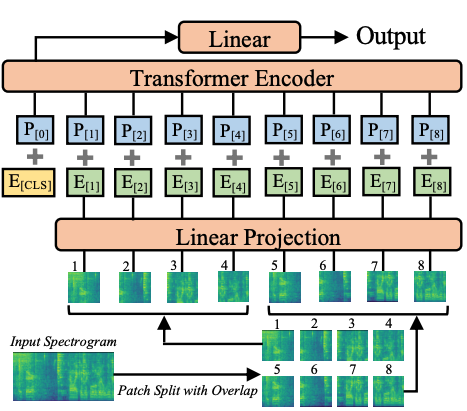
\includegraphics[trim=0 0 0 116, clip, scale=0.7]{figures/patchembedding.png}
    \caption{Creation of a sequence of patch embeddings from an input spectrogram. The spectrogram is split into overlapping patches, each of which is linearly projected into a one-dimensional embedding vector. A learnable positional embedding is then added to each patch embedding. An initial \acrfull{CLS} is also included, as is common in classification tasks~\cite{gong2021astaudiospectrogramtransformer}.}
    \label{PatchEmbeddingFigure}
\end{figure}

\subsection{Architecture Modifications}

The original Vision Transformer was designed for classification tasks, where the output is a single vector rather than a sequence. In contrast, \gls{ADT} is a sequence labeling task, requiring an output sequence whose temporal resolution matches that of the input.

To accommodate this, we reinterpret groups of patch embeddings as representing individual time frames. This is feasible as long as the number of timesteps divides evenly into the total number of patches, allowing the output to be reshaped to match the desired sequence length.

Since we do not perform classification, the additional \gls{CLS} typically used to summarize the input for class prediction (as seen in Figure~\ref{PatchEmbeddingFigure}) is unnecessary and thus omitted~\cite{dosovitskiy2021imageworth16x16words}.

\subsection{Implementation}

I implemented the Vision Transformer by first converting the input spectrogram into a sequence of patch embeddings with shape $(T \times D_e)$. This is done using a 2D convolutional layer with kernel size and stride equal to the patch size $(1 \times P)$, where $P$ is the patch height. This value is chosen such that the spectrogram's 84 frequency bins can be evenly divided into $n_P = \frac{84}{P}$ patches. To control the output embedding dimensionality $D_e$, the convolution uses $\frac{D_e}{n_P}$ kernels.

Since each patch has a width of 1, it retains information only about the frequencies within its own time frame, helping preserve the temporal resolution of the input spectrogram. A learnable positional embedding of shape $(\frac{D_e}{n_P} \times n_P)$ is then added to each patch to encode spectral position and kernel identity. These patches are then permuted and flattened into a sequence, forming the final patch embedding representation.

While each patch embedding encodes its relative position within a time frame, it lacks information about which time frame it belongs to. To introduce this temporal ordering, I add a sinusoidal positional encoding across the time dimension. The resulting sequence is then passed through $L$ transformer blocks with pre-layer normalization and multi-head self-attention using $H$ heads, following the same design as in the convolutional transformer. Finally, a linear output layer computes onset probabilities for each of the five drum instruments. This full architecture is illustrated in Figure~\ref{ViTFigure}, with its corresponding tunable hyperparameters described in Table~\ref{ViTHyperparams}.

\begin{figure}[H]
    \hspace*{-0.5cm}
    \centering
    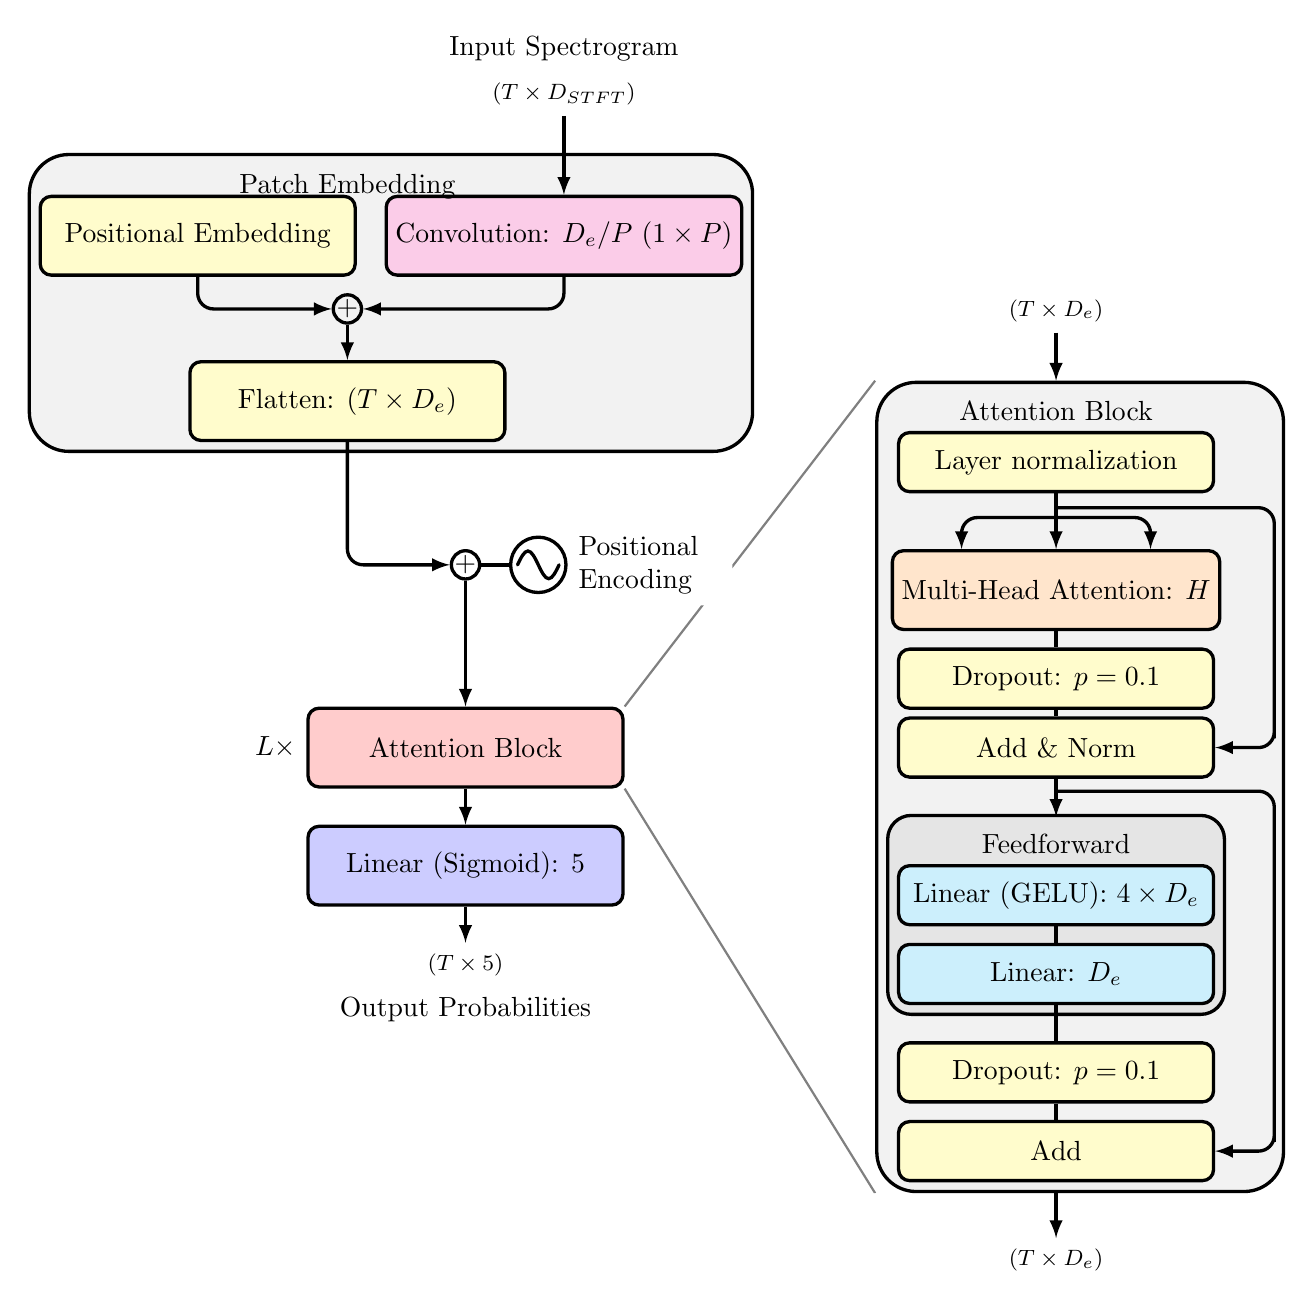
\begin{tikzpicture}[
    very thick,
    arrow/.style={
        -latex,
        very thick,
        rounded corners=0.2cm
    },
    do path picture/.style={%
        path picture={%
          \pgfpointdiff{\pgfpointanchor{path picture bounding box}{south west}}%
            {\pgfpointanchor{path picture bounding box}{north east}}%
          \pgfgetlastxy\x\y%
          \tikzset{x=\x/2,y=\y/2}%
          #1
        }
    },
    sin wave/.style={do path picture={    
        \draw [line cap=round] (-3/4,0)
        sin (-3/8,1/2) cos (0,0) sin (3/8,-1/2) cos (3/4,0);
        }
    }
    ]

\node[anchor=south, label=above:{Input Spectrogram}] at (1.25, -0.5){\footnotesize{($T \times D_\text{STFT}$)}};

\draw[arrow] (1.25, -0.5) -- (1.25, -1.5) node [rectangle,
rounded corners,
draw,
anchor=north,
fill=magenta!20,
minimum height=1cm,
minimum width=4cm
] (a) {Convolution: $D_e/P$ $(1 \times P)$};

\node [rectangle,
rounded corners,
draw,
anchor=north,
fill=yellow!20,
minimum height=1cm,
minimum width=4cm,
left = 1em of a,
] (b) {Positional Embedding};

\node[circle, 
draw, 
anchor=north,
minimum size=1em, 
inner sep=0pt
] at (-1.5, -2.75) (c) {$\mathbf{+}$};

\draw[arrow] (b) |- (c.west);
\draw[arrow] (a) |- (c.east);

\draw [arrow] (c) -- (-1.5, -3.6) node [rectangle,
rounded corners,
draw,
anchor=north,
fill=yellow!20,
minimum height=1cm,
minimum width=4cm,
] (d) {Flatten: $(T \times D_e)$};

\node [anchor=north,
above = 3em of c,
] (e) {Patch Embedding};

\begin{scope}[on background layer]
    \node[rectangle,
    fill=gray!10,
    rounded corners=5mm,
    draw,
    very thick,
    fit= (a) (b) (d) (e)] {};
\end{scope}

\node[circle, 
draw, 
anchor=north,
minimum size=1em, 
inner sep=0pt
] at (0, -6) (h) {$\mathbf{+}$};

\draw[arrow] (d) |- (h);

\node [circle, 
draw, 
sin wave, 
minimum size=2em, 
right=1em of h,
label={[align=left]east:Positional\\Encoding}
] (pe) {};

\draw (pe) -- (h);

\draw[arrow] (h) -- (0, -8) node[rectangle,
rounded corners,
draw,
anchor=north,
minimum size=1em,
inner sep=0pt,
fill=red!20,
minimum height=1cm,
minimum width=4cm,
label={west:$L\times$}
] (v) {Attention Block};

\draw[arrow] (v) -- (0, -9.5) node[rectangle, 
rounded corners, 
draw, 
anchor=north, 
fill=blue!20,
minimum height=1cm,
minimum width=4cm
] (w) {Linear (Sigmoid): $5$};

\draw[arrow] (w) -- (0, -11.0);

\node[anchor=north, label=below:{Output Probabilities}] at (0, -11.0){\footnotesize{($T \times 5$)}};


% ---- Attention Block ----
\draw (7.5, -4.5) node[rectangle,
rounded corners,
draw,
anchor=north,
fill=yellow!20,
label=north:Attention Block,
minimum height=0.75cm,
minimum width=4cm
] (i) {Layer normalization};

\draw[arrow] (i) -- (7.5, -6) node [rectangle,
rounded corners,
draw,
anchor=north,
fill=orange!20,
minimum height=1cm,
minimum width=4cm
] (j) {Multi-Head Attention: $H$};

\draw[arrow] (j.north)++(0, 0.4) -| ($(j.north) + (1.2,0)$);
\draw[arrow] (j.north)++(0, 0.4) -| ($(j.north) + (-1.2,0)$);

\draw (j) -- (7.5, -7.25) node[rectangle,
rounded corners,
draw,
anchor=north,
fill=yellow!20,
minimum height=0.75cm,
minimum width=4cm
] (k) {Dropout: $p = 0.1$};

\draw (k) -- (7.5, -8.125) node[rectangle,
rounded corners,
draw,
anchor=north,
fill=yellow!20,
minimum height=0.75cm,
minimum width=4cm
] (l) {Add \& Norm};

\coordinate (larrow) at ($(l.east) + (0.75, 0)$);
\draw[arrow] (j.north)++(0, 0.525) -| (larrow) |- (l.east);

\node[rectangle,
rounded corners,
draw,
anchor=north,
fill=cyan!20,
minimum height=0.75cm,
minimum width=4cm
] at (7.5, -10) (m) {Linear (GELU): $4 \times D_e$};

\coordinate (m1) at ($(m.north) + (0, 0.5)$);
\draw[arrow] (l) -- ($(m1.north) + (0, 0.1)$);

\draw (m) -- (7.5, -11) node[rectangle,
rounded corners,
draw,
anchor=north,
fill=cyan!20,
minimum height=0.75cm,
minimum width=4cm
] (n) {Linear: $D_e$};

\draw (n) -- (7.5, -12.25) node[rectangle,
rounded corners,
draw,
anchor=north,
fill=yellow!20,
minimum height=0.75cm,
minimum width=4cm
] (o) {Dropout: $p = 0.1$};

\draw (o) -- (7.5, -13.25) node[rectangle,
rounded corners,
draw,
anchor=north,
fill=yellow!20,
minimum height=0.75cm,
minimum width=4cm
] (p) {Add};

\draw[arrow] (m.north)++(0, 0.925) -| ($(p.east) + (0.75, 0)$) |- (p.east);

\coordinate (i1) at ($(i.north) + (0, 0.5)$);

\begin{scope}[on background layer]

    \node[rectangle,
    fill=gray!20,
    rounded corners=3mm,
    label={[name=mnlabel, yshift=-0.625cm]north:Feedforward},
    draw,
    very thick,
    fit=(m) (m1) (n)] (mn) {};
    \node[rectangle,
    fill=gray!10,
    rounded corners=5mm,
    draw,
    very thick,
    fit= (i1) (mn) (p) (larrow)] (imnp) {};
    \node[rectangle,
    fill=gray!20,
    rounded corners=3mm,
    label={[name=mnlabel, yshift=-0.625cm]north:Feedforward},
    draw,
    very thick,
    fit=(m) (m1) (n)] (mn) {};

    \begin{scope}[even odd rule]
        \path[clip] 
        (current bounding box.south west) rectangle (current bounding box.north east)
        ($(pe.north east) + (0, 0.25)$) rectangle ($(pe.south east) + (2.2, -0.25)$);
        \draw[thick, color=black!50] (v.north east) -- (imnp.north west);
        \draw[thick, color=black!50] (v.south east) -- (imnp.south west);
      \end{scope}
\end{scope};

\draw[arrow] (7.5, -3.25) node[anchor=south] {\footnotesize{($T \times D_e$)}} -- (i |- imnp.north);
\draw[arrow] (p |- imnp.south) -- (7.5, -14.75) node[anchor=north] {\footnotesize{($T \times D_e$)}};

\end{tikzpicture}
    \caption{Model architecture of the Vision Transformer used in this thesis.}
    \label{ViTFigure}
\end{figure}

\begin{table}[H]
    \centering
    \begin{tabular}{lr|c}
        \multicolumn{2}{c|}{Hyperparameter} & Values       \\
        \hline
        $P$ & Patch height      & \{7, 14, 21\} \\
        $H$ & Number of heads     & \{2, 4, 6, 8\} \\
        $L$ & Number of layers      & \{2, 4, 6, 8, 10\} \\
        $D_e$ & Embedding dimension      & \{72, 144, 288, 576\} \\
    \end{tabular}
    \caption{Hyperparameters and their corresponding search spaces for training the Vision Transformer.}
    \label{ViTHyperparams}
\end{table}